\documentclass[mathserif]{beamer}
\newcommand{\be}{\begin{equation}}
\newcommand{\ee}{\end{equation}}
\newcommand{\bce}{\begin{center}}
\newcommand{\ece}{\end{center}}
\newcommand{\dpa}[2]{\frac{\partial #1}{\partial #2}}
\newcommand{\ndp}[3]{\frac{\partial^#3 #1}{\partial #2 ^#3}}
\newcommand{\cdpa}[3]{\frac{\partial^2 #1}{\partial #2 \partial #3}}
\usepackage[utf8]{inputenc}
\usepackage{ragged2e}
\usepackage{etoolbox}
\usepackage{animate}
\usepackage{booktabs}
\usepackage{eulervm}
\apptocmd{\frame}{}{\justifying}{}
\usepackage[activeacute,spanish]{babel}
\setbeamertemplate{navigation symbols}{}
\setbeamertemplate{caption}[numbered]
\usetheme{default}
\setbeamertemplate{footline}[frame number]
\usecolortheme[named=purple]{structure}
\setbeamercolor{alerted text}{fg=blue}
\title{Acoplamiento Meso-Microescala Utilizando WRF-LES Para la Simulación Numérica de Viento Sobre Terreno Complejo de Alta Resolución}
\author{P.~Cárdenas, A.~Flores}
\institute[Universidad Técnica Federico Santa María]
{%
  Departamento de Ing. Mecánica\\
  Universidad Técnica Federico Santa María}
\date{XVI Jornadas de Mecánica Computacional, 2017}
\AtBeginSubsection[]
{
  \begin{frame}<beamer>{Outline}
    \tableofcontents[currentsection,currentsubsection]
  \end{frame}
}
\begin{document}
\begin{frame}
  \titlepage
\end{frame}

\begin{frame}{Contenidos}
	\tableofcontents
\end{frame}

\section{1. Objetivos}
\begin{frame}{Objetivos}
	\begin{block}{Objetivo Principal}\justifying
	   	Estudiar el rendimiento del modelo WRF mesoescala al resolver los fenómenos turbulentos de microescala desarrollados en la CLP en su interacción con el terreno complejo aplicando un modelo LES-TKE de orden 1.5 para asi poder estimar el comportamiento del viento en zonas de alto potencial eólico.
	\end{block}
	\begin{block}{Objetivo Secundario}\justifying
		Mejorar este rendimiento mediante el uso de asimilación de información y análisis variacional de data a alta resolución en las condiciones de contorno.
	\end{block}
\end{frame}

\section{2. Motivación}
\begin{frame}{Motivación}{Estimación Eólica}
	\begin{figure}[H]
		\centering
		\includegraphics[width=0.9\linewidth,trim={5.4cm 2cm 15cm 5.5cm},clip]{explorador}
		\caption{Información del Explorador Eólico para la zona de interés.}
		\label{fig:explorador}
	\end{figure}
\end{frame}

\begin{frame}{Motivación}{Simulaciones Multiescala}
	\begin{figure}[H]
		\centering
		\includegraphics[width=0.7\linewidth]{terraincog}
		\caption{Separación de escalas en simulación de mecánica de fluidos.}
		\label{fig:escalas}
	\end{figure}
\end{frame}

\section{3. Metodología}
\begin{frame}{Metodología}{WRF}
	\begin{itemize}\justifying
		\item \emph{Weather Research and Forecasting Model}.
		\item Modelo comunitario, open source, gratis, con desarrollo distribuido y soporte centralizado.
		\item Su desarrollo lo lidera NCAR y NOAA, en colaboración con distintas universidades en el mundo.
		\item Resuelve las ecuaciones dinámicas de la atmósfera utilizando un sistema Eureliano con coordenadas verticales que siguen el terreno.
	\end{itemize}
	
	\begin{equation}
	\eta = \frac{p_{dh}-p_{dht}}{p_{dhs} - p_{dht}} = \frac{p_{dh}-p_{dht}}{\mu_d}
	\end{equation}
\end{frame}

\begin{frame}{Metodología}{WRF}
	\begin{figure}[H]
		\centering
		\includegraphics[width=0.55\linewidth,trim={11.5cm 3.3cm 1cm 14cm},clip]{eta}
		\caption{Estructura de la coordenada vertical.}
		\label{fig:eta}
	\end{figure}
\end{frame}

\begin{frame}{Metodología}{Ecuaciones}
Se resuelven las ecuaciones de Euler:
\begin{align} \partial_t U + (\nabla\cdot\vec{V}u)-\partial_x(p\phi_\eta) + \partial_\eta (p\phi_x) &= F_U \\
\partial_t V + (\nabla\cdot\vec{V}v)-\partial_y(p\phi_\eta) + \partial_\eta (p\phi_y) &= F_V \\
\partial_t W + (\nabla\cdot\vec{V}w)- g(\partial_\eta p - \mu) &= F_W \\
\partial_t\Theta + (\nabla\cdot \vec{V}\theta) &= F_\Theta \\
\partial_t\mu + (\nabla\cdot \vec{V})&= 0 \\
\partial_t\phi + \mu^{-1}[(\vec{V}\cdot\nabla\phi)-gW] &= 0
\end{align}
Ademas de la relación auxiliar y la ecuación de estado:
\be \partial_\eta\phi = -\alpha\mu \ee 
\be p = p_0 \left( \frac{R_d\theta}{p_0\alpha} \right)^\gamma \ee

Estas ecuaciones son referenciales!
\end{frame}

\begin{frame}{Metodología}{Parametrizaciones}
Debido a la resolución del modelo, los fenómenos que la malla no alcanza a resolver deben ser parametrizados. Cada uno de estos términos se agrega al lado derecho de la ecuación de Euler.

Estos son:

	\begin{itemize}
		\item Microfísica
		\item Cúmulos
		\item Capa Límite Planetaria
		\item Capa Superficial
		\item Modelo de Suelo
		\item Radiación
	\end{itemize}
\end{frame}

\begin{frame}{Metodología}{Parametrizaciones}
	\begin{figure}[H]
		\centering
		\includegraphics[width=0.95\linewidth]{param}
		\caption{Esquema de interacción entre los fenómenos.}
		\label{fig:param}
	\end{figure}
\end{frame}

\begin{frame}{Metodología}{Turbulencia}
WRF separa la difusión (turbulenta) vertical de la horizontal. 

La difusión horizontal es resuelta explícitamente según el modelo de viscosidad turbulenta a utilizar, mientra que la difusión vertical se parametriza en los esquemas de CLP.

{\small
\begin{eqnarray}
\partial_t U = \ldots - m_x[\partial_x\tau_{11}+\partial_y\tau_{12}-\partial_z(z_x\tau_{11}+z_y\tau_{12})]-\partial_z\tau_{13} \\
\partial_t V = \ldots - m_y[\partial_x\tau_{12}+\partial_y\tau_{22}-\partial_z(z_x\tau_{12}+z_y\tau_{22})]-\partial_z\tau_{23} \\
\partial_t W = \ldots - m_y[\partial_x\tau_{13}+\partial_y\tau_{23}-\partial_z(z_x\tau_{13}+z_y\tau_{23})]-\partial_z\tau_{33}
\end{eqnarray}}

\begin{equation}
\tau_{ij} = -\mu_d K_{h,v}D_{ij}
\end{equation}

La forma de determinar $K_{h,v}$ define el LES.
\end{frame}

\begin{frame}{Metodología}{Turbulencia}
Para las malla no LES:
\begin{equation}
K_h = C_s^2 l^2[0.25(D_{11}-D_{22})^2+D_{12}]^{0.5}
\end{equation}
Con $C_s=0.25$ y $l=\sqrt{\Delta x\Delta y}$

\bigskip
Para las mallas LES:
\begin{equation}
K_{h,v} = C_k l_{h,v}\sqrt{e}
\end{equation}

Con $0.15\leq C_k \leq 0.25$. Como se presume anisotrópico:
\begin{align}
l_v &= \min[\Delta z, 0.76\sqrt{e}/N]\quad&;&\quad N^2>0\\
l_h &= \Delta z\quad&;&\quad N^2\leq 0
\end{align}
$N$ es la frecuencia de Brunt-Väisälä. $N=\sqrt{g/\theta d_z\theta}$
\end{frame}

\begin{frame}{Metodología}{Clausura TKE 1.5}
	Se introduce una ecuación de transporte para $e$ de la forma:
	\bigskip
	
	{\footnotesize
	\begin{equation}
	\partial_t(\mu_d e) + (\partial_i V_i e)_\eta = \mu_d(\text{producción + flotación + disipación})
	\end{equation}}

{\small
	\begin{align}
	\text{producción}&= K_h (D_{11}^2 + D_{22}^2 + D_{12}^2) + K_v (D_{33}^2 + D_{13}^2 + D_{23}^2)\\
	\text{flotación}&=-K_v N^2\\
	\text{disipación}&=-\frac{C e^{3/2}}{l}
	\end{align}}
Con:
{\small
\begin{align}
C &= 1.9C_k + \frac{(0.93 - 1.9 C_k)l}{(\Delta x \Delta y \Delta z)^{1/3}}\\
l &= \min[(\Delta x \Delta y \Delta z)^{1/3}, 0.76\sqrt{e}/N]
\end{align}}
\end{frame}
%\begin{frame}{Metodología}{Aspectos Numéricos}
%	\begin{itemize}
%		\item Coordenada Vertical
%		\item Malla staggered
%		\item Esquema RK3 para integración temporal
%		\item Filtro acústico para ondas de presión
%		\item Anidamiento de dominios
%	\end{itemize}
%\end{frame}

\section{4. Caso de Estudio}
\begin{frame}{Caso de Estudio}{Dominios y Resolución Espacial}
	\begin{itemize}\justifying
		\item La malla numérica consta de 6 mallas anidadas telescópicamente y centradas en Punta Curaumilla (-33.097344, -71730552).
		\item Cada malla consta de $121\times121\times47$ nodos.
		\item $\Delta x=\Delta y =12150\rightarrow4050\rightarrow1350\rightarrow450\rightarrow150\rightarrow50$
	\end{itemize}
	\begin{figure}[H]
		\begin{minipage}{0.5\textwidth}
			\begin{itemize}\justifying\vspace{-12mm}
		\item Las últimas 3 mallas: LES.
		\item La malla vertical se fabrica de tal forma que se capture el comportamiento dentro de la capa límite.
		\item Se utiliza un $\Delta t = 12$ [s] para iterar en la malla mas gruesa. De esta forma no se viola la condición CFL.
	\end{itemize}
	\end{minipage}%
	\begin{minipage}{0.5\textwidth}
		\centering
		\includegraphics[width=\linewidth,page=9,trim={1cm 6cm 4cm 7.85cm},clip]{perfil_medio}
		\vspace{-2mm}
		\caption{Distribución malla vertical.}
		\label{fig:vertical_mesh}
	\end{minipage}%
	\end{figure}
\end{frame}

\begin{frame}{Caso de Estudio}{Dominios y Resolución Espacial}
	\begin{figure}[H]
		\centering
		\includegraphics[width=0.95\linewidth]{d06d05}
		\caption{Dominios de las mallas exteriores d01 y d02.}
		\label{fig:0102}
	\end{figure}
\end{frame}

\begin{frame}{Caso de Estudio}{Dominios y Resolución Espacial}
	\begin{figure}[H]
		\centering
		\includegraphics[width=0.95\linewidth]{d05d04}
		\caption{Dominios de las mallas exteriores d02 y d03.}
		\label{fig:0203}
	\end{figure}
\end{frame}

\begin{frame}{Caso de Estudio}{Dominios y Resolución Espacial}
	\begin{figure}[H]
		\centering
		\includegraphics[width=0.95\linewidth]{d04d03}
		\caption{Dominios de las mallas exteriores d03 y d04.}
		\label{fig:0304}
	\end{figure}
\end{frame}

\begin{frame}{Caso de Estudio}{Dominios y Resolución Espacial}
	\begin{figure}[H]
		\centering
		\includegraphics[width=0.95\linewidth]{d03d02}
		\caption{Dominios de las mallas exteriores d04 y d05.}
		\label{fig:0405}
	\end{figure}
\end{frame}

\begin{frame}{Caso de Estudio}{Dominios y Resolución Espacial}
	\begin{figure}[H]
		\centering
		\includegraphics[width=0.95\linewidth]{d02d01}
		\caption{Dominios de las mallas exteriores d05 y d06.}
		\label{fig:0506}
	\end{figure}
\end{frame}

\begin{frame}{Caso de Estudio}{Dominios y Resolución Espacial}
	\vspace{4mm}
	\begin{figure}[H]
		\centering
		\includegraphics[width=0.75\linewidth,trim={1cm 6.5cm -1cm 4cm},clip]{altura}
		\vspace{-3mm}
		\caption{Puntos de monitoreo dominio d06.}
		\label{fig:monitor}
	\end{figure}
\end{frame}

\begin{frame}{Caso de Estudio}{CB e Información del Terreno}
	\begin{itemize}\justifying
		\item Las condiciones de borde provienen del modelo GFS global con una resolución de $0,5^\circ \approx 55,6$ [km].
		\item La coordenada de presión se fija a $p_{dht} = 5000$ [kPa].
		\item La información de la topografía se interpola de los datos obtenidos por la operación del satélite STRM de la NASA con 3'' de resolución $\approx 90$ [m].
		\item La información para el uso de suelo y otras características del terreno se obtienen a través de los instrumentos satelitales MODIS.
		\item Se modelan 12 horas del 10/01/2010.
	\end{itemize}
\end{frame}

\begin{frame}{Caso de Estudio}{Parametrizaciones}
\begin{table}[h!]
	\caption{Esquemas de Parametrización Utilizados.}\label{tab:esquemas}
	\centering
	{\footnotesize \begin{tabular}{lllllll}
		\toprule
		Física 					& d01	&	d02	&	d03	&	d04	&	d05	&	d06 \\
		\midrule
		Micro-físicas		 	& WSM5 & WSM5 & WSM5 &WSM5&WSM5&WSM5  \\
		Cúmulos			 		& Grell & -- & -- & -- & -- & -- \\ 
		Capa Superf.	 	& MM5 & MM5 & MM5 & MM5 & MM5 & MM5 \\
		PBL				 		& YSU & YSU & YSU & -- & -- & -- \\
		Modelo Suelo 		& Dif. & Dif. & Dif. & Dif. & Dif. & Dif. 	\\
		Rad. Larga	& RRTM &RRTM&RRTM&RRTM&RRTM&RRTM \\
		Rad. Corta	& Dudhia &Dudhia&Dudhia&Dudhia&Dudhia&Dudhia \\
		\bottomrule
	\end{tabular}}
\end{table}
\end{frame}

\section{5. Resultados}
\begin{frame}{Resultados}{Series de Tiempo}
	\begin{figure}[H]
	\centering
	\begin{tabular}{cc}
		\begin{tabular}{c}\includegraphics[width=0.44\linewidth,page=11,trim={2cm 6cm 4cm 8cm},clip]{u_ts}\end{tabular}\hspace{-1cm}&
		\begin{tabular}{c}\includegraphics[width=0.44\linewidth,page=12,trim={2cm 6cm 4cm 8cm},clip]{u_ts}\end{tabular}\\
	\end{tabular}
	\caption{Rapidez y Ángulo del viento para $\eta_l=6, z_l=123.349$ [m]}
	\label{ts_ang}
	\end{figure}
\end{frame}

\begin{frame}{Resultados}{Viento Superficial}
\vspace{-1cm}
\begin{center}
\animategraphics[loop,controls,width=0.63\linewidth]{12}{ani/rapidez_ins_10m.}{1}{37}
\end{center}
\end{frame}

\begin{frame}{Resultados}{Viento Medio}
	\begin{figure}[H]
		\centering%\vspace{-0.3cm}
		\begin{tabular}{ccc}
			\scriptsize $\overline{z}=8.20464$ [m]&\hspace{-1cm}\scriptsize $\overline{z}=24.6166$ [m] &\hspace{-1cm}\scriptsize $\overline{z}=38.9816$ [m]\\
			\begin{tabular}{c}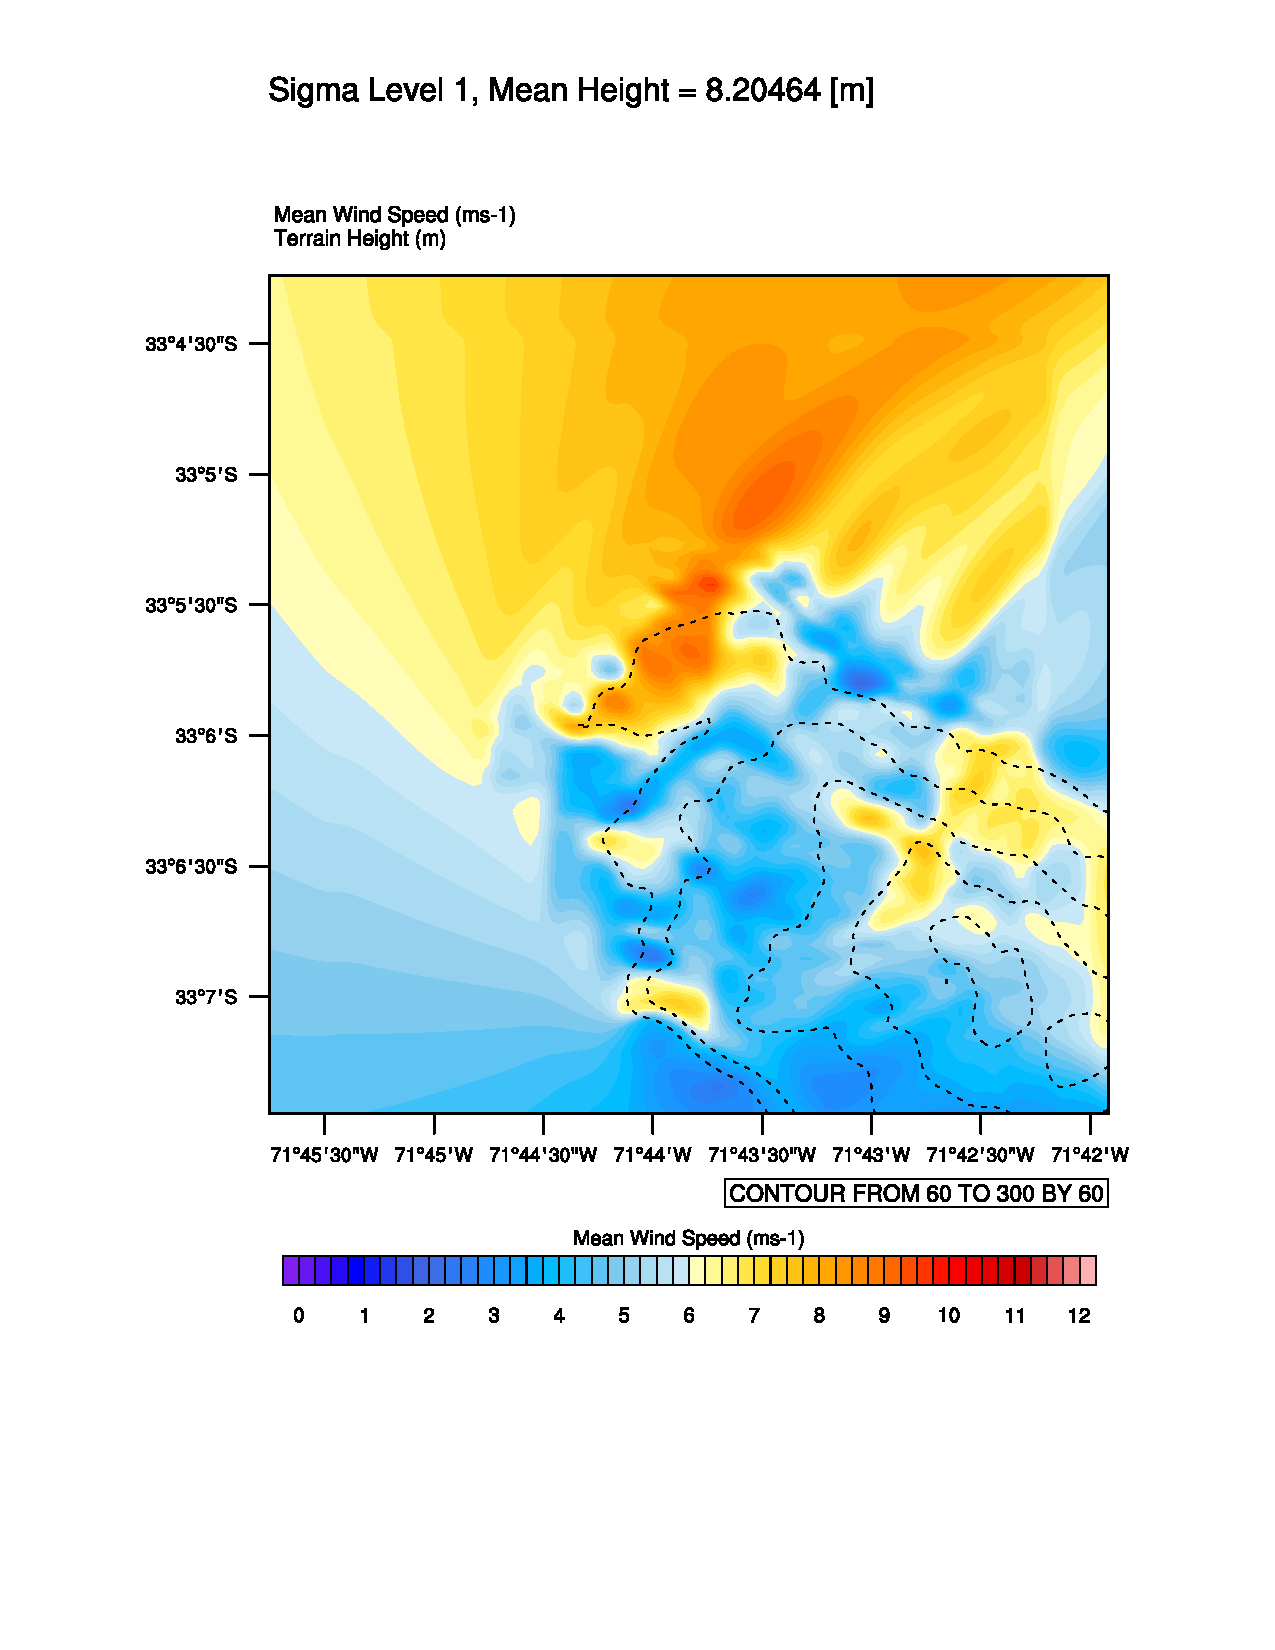
\includegraphics[width=0.3\linewidth,page=1,trim={2cm 5.5cm 1cm 4.5cm},clip]{rapidez_media}\end{tabular}&\hspace{-1cm}
			\begin{tabular}{c}\includegraphics[width=0.3\linewidth,page=2,trim={2cm 5.5cm 1cm 4.5cm},clip]{rapidez_media}\end{tabular}&\hspace{-1cm}
			\begin{tabular}{c}\includegraphics[width=0.3\linewidth,page=3,trim={2cm 5.5cm 1cm 4.5cm},clip]{rapidez_media}\end{tabular}\\
			\scriptsize $\overline{z}=51.2991$ [m]&\hspace{-1cm}\scriptsize $\overline{z}=82.144$ [m] &\hspace{-1cm}\scriptsize $\overline{z}=123.349$ [m]\\
			\begin{tabular}{c}\includegraphics[width=0.3\linewidth,page=4,trim={2cm 5.5cm 1cm 4.5cm},clip]{rapidez_media}\end{tabular}&\hspace{-1cm}
			\begin{tabular}{c}\includegraphics[width=0.3\linewidth,page=5,trim={2cm 5.5cm 1cm 4.5cm},clip]{rapidez_media}\end{tabular}&\hspace{-1cm}
			\begin{tabular}{c}\includegraphics[width=0.3\linewidth,page=6,trim={2cm 5.5cm 1cm 4.5cm},clip]{rapidez_media}\end{tabular}\\
		\end{tabular}
		\vspace{-2mm}
		\caption{Rapidez del viento medio para los primeros 6 niveles verticales.}
		\label{med_wind}
	\end{figure}
\end{frame}

\begin{frame}{Resultados}{Perfiles de Viento}
	\begin{figure}[H]
	\centering
	\begin{tabular}{cc}
		\begin{tabular}{c}\includegraphics[width=0.38\linewidth,page=1,trim={2cm 6cm 2cm 7.6cm},clip]{perfil_medio}\end{tabular}&\hspace{-1cm}
		\begin{tabular}{c}\includegraphics[width=0.38\linewidth,page=3,trim={2cm 6cm 2cm 7.6cm},clip]{perfil_medio}\end{tabular}\\
		\begin{tabular}{c}\includegraphics[width=0.38\linewidth,page=5,trim={2cm 6cm 2cm 7.6cm},clip]{perfil_medio}\end{tabular}&\hspace{-1cm}
		\begin{tabular}{c}\includegraphics[width=0.38\linewidth,page=7,trim={2cm 6cm 2cm 7.6cm},clip]{perfil_medio}\end{tabular}\\
	\end{tabular}
	%\vspace{-4mm}
	\caption{Perfiles de viento promedio para los puntos de observación.}
	\label{perf_wind}
	\end{figure}
\end{frame}

\begin{frame}{Resultados}{Espectros}
	\begin{figure}[H]
		\centering\vspace{-0.4cm}
		\begin{tabular}{cc}
			\scriptsize $\overline{z}=8.20464$ [m]&\hspace{-1cm}\scriptsize $\overline{z}=164.752$ [m]\\
			\begin{tabular}{c}\includegraphics[width=0.44\linewidth,page=1,trim={0cm 0cm 0cm 1.4cm},clip]{spectra}\end{tabular}&\hspace{-1cm}
			\begin{tabular}{c}\includegraphics[width=0.44\linewidth,page=7,trim={0cm 0cm 0cm 1.4cm},clip]{spectra}\end{tabular}\\
			\scriptsize $\overline{z}=277.528$ [m]&\hspace{-1cm}\scriptsize $\overline{z}=1189.48$ [m]\\
			\begin{tabular}{c}\includegraphics[width=0.44\linewidth,page=9,trim={0cm 0cm 0cm 1.4cm},clip]{spectra}\end{tabular}&\hspace{-1cm}
			\begin{tabular}{c}\includegraphics[width=0.44\linewidth,page=14,trim={0cm 0cm 0cm 1.4cm},clip]{spectra}\end{tabular}\\
		\end{tabular}
		\vspace{-2mm}
		\caption{Espectro de velocidad horizontal para los niveles 1, 7, 9 y 14.}
		\label{spectra_wind}
	\end{figure}
\end{frame}

\section{4. Conclusiones y Trabajo Futuro}
\begin{frame}{Conclusiones}{Análisis}
\begin{itemize}\justifying
  \item Existe concordancia física entre lo simulado y lo real, mostrando una aceleración, separación, recirculación y  \emph{reattachment} debido a la pendiente natural del sitio.
  \item WRF muestra un buen rendimiento para este tipo de simulaciones, siempre y cuando los datos de entrada tengan la resolución necesaria.
  \item El terreno complejo afecta en gran medida el comportamiento del flujo, la estimación eólica en este tipo de zonas debe ser mas detallada.
  \item Los perfiles de velocidad y los espectros de energía se comportan según lo esperado.
\end{itemize}
\end{frame}

\begin{frame}{Conclusiones}{Trabajo Futuro}
	\begin{itemize}\justifying
		\item Este tipo de simulaciones son muy costosas computacionalmente. Se espera optimizar el código para mejorar su eficiencia.
		\item Para convencernos: probar otros esquemas LES, sensibilidad a las CB, parametrizaciones, etc.
		\item Se necesita validación de los datos:
		\begin{itemize}
			\item Obtención de datos experimentales con globos meteorológicos.
			\item Implementación de Data Assimilation.
			\item Simulación caso Bolund (benchmark para terreno complejo).
		\end{itemize}
	\end{itemize}
\end{frame}

\begin{frame}
  \titlepage
\end{frame}

\end{document} 